%% The first command in your LaTeX source must be the \documentclass command.
%%
%% Options:
%% twocolumn : Two column layout.
%% hf: enable header and footer.
\documentclass[
% twocolumn,
% hf,
]{ceurart}

%%
%% One can fix some overfulls
\sloppy

%%
%% Minted listings support 
%% Need pygment <http://pygments.org/> <http://pypi.python.org/pypi/Pygments>
\usepackage{listings}
\usepackage{lmodern}
\usepackage{minted}
\usepackage{textcomp}

%\usepackage[breakable]{tcolorbox}
%\usepackage{enumerate} % Needed for markdown enumerations to work
%\usepackage{geometry} % Used to adjust the document margins
%\usepackage{upquote} % Upright quotes for verbatim code
%\usepackage{eurosym} % defines \euro
%\usepackage[mathletters]{ucs} % Extended unicode (utf-8) support
%\usepackage{fancyvrb} % verbatim replacement that allows latex
%\usepackage{grffile} % extends the file name processing of package graphics % to support a larger range

%% auto break lines
\lstset{breaklines=true}

%%
%% end of the preamble, start of the body of the document source.
\begin{document}

%%
%% Rights management information.
%% CC-BY is default license.
\copyrightyear{2022}
\copyrightclause{Copyright for this paper by its authors.
  Use permitted under Creative Commons License Attribution 4.0
  International (CC BY 4.0).}

%%
%% This command is for the conference information
\conference{IJCAI-ECAI 2022, the 31st International Joint Conference on Artificial Intelligence and the 25th European Conference on Artificial Intelligence, July 23-29, 2022
Messe Wien, Vienna, Austria}

%%
%% The "title" command
\title{Understand your clusters: a link between the data and metadata}

\tnotemark[1]
\tnotetext[1]{You can use this document as the template for preparing your
  publication. We recommend using the latest version of the ceurart style.}

%%
%% The "author" command and its associated commands are used to define
%% the authors and their affiliations.
\author[1,2]{Dmitry S. Kulyabov}[%
orcid=0000-0002-0877-7063,
email=kulyabov-ds@rudn.ru,
url=https://yamadharma.github.io/,
]
\cormark[1]
\fnmark[1]
\address[1]{Peoples' Friendship University of Russia (RUDN University),
  6 Miklukho-Maklaya St, Moscow, 117198, Russian Federation}
\address[2]{Joint Institute for Nuclear Research,
  6 Joliot-Curie, Dubna, Moscow region, 141980, Russian Federation}

\author[3]{Ilaria Tiddi}[%
orcid=0000-0001-7116-9338,
email=i.tiddi@vu.nl,
url=https://kmitd.github.io/ilaria/,
]
\fnmark[1]
\address[3]{Vrije Universiteit Amsterdam, De Boelelaan 1105, 1081 HV Amsterdam, The Netherlands}

%% Footnotes
\cortext[1]{Corresponding author.}
\fntext[1]{These authors contributed equally.}

%%
%% The abstract is a short summary of the work to be presented in the
%% article.
\begin{abstract}
  In this preliminary work we present an approach for clustering augmented with Natural Language Explanations.
  With clustering there are 2 main challenges: a) choice of proper, reasonable number of clusters and b) cluster profiling.
  There is a plethora of technics for a) but not so much for b), which is in general laborious task of explaining obtained clusters.
  Clustering is in a sense art in that regard that it is intuitive and iterative process.
  Therefore, XAI techniques are well suited in this area.
  On a convincing example we show how process of clustering on a set of "objective" variables could be facilitated with textual metadata.
  In our case images of products from online fashion store are used for clustering.
  Then product descriptions are used for profiling clusters.
\end{abstract}

%%
%% Keywords. The author(s) should pick words that accurately describe
%% the work being presented. Separate the keywords with commas.
\begin{keywords}
  XAI \sep
  NLU \sep
  clustering \sep
  TODO
\end{keywords}

%%
%% This command processes the author and affiliation and title
%% information and builds the first part of the formatted document.
\maketitle

\section{Introduction}
%In general what is the prroblem -- in clustering we need to analyse results, XAI can help us in doing that
%- classification as a tool for understanding
Categorization is a one of ways how humans describe the world.
To classify means to notice that some phenomenas differ from each other.
And more importantly how they differ.
Finally, one is giving names to those different classes of entities.
Clustering in machine learning in an essence is no different process.

%- the problem is common in fields like: marketing, e-commerce, industries, ???
%- one like to classify "objective" data like images, sensors, etc to uncover hidden structure
%- to many observations to do it manually
Clustering methods are common in many fields of human prosperity.
In the advent of an ever-increasing amount of data, we use tools to automate the process, as manual clustering is too laborious.
Indeed, there are many statistical, machine learning and deep learning algorithms.
The difficulty arises to convince end-user that derived clusters make sense.
Will it be clustering sensors data in Industry 4.0 or behaviours of consumers, results needs to be actionable.
We believe that this is not possible if we do not explain what algorithm has learned. % and if it is of any value for human.
It also follows that the process is iterative.
We continually hypothesize about the significant differences between classes, then test results by looking at classified objects.

%- explanations needs to be done with data comprehensible by humans
%   - data are not equal
%  - images are self-explanatory in e-commerce setting, but not necessarily in other (vide images of medical images, satellites,  etc)
%  - industrial data - rarely
%  - thus "metadata" - link between "objective/hard" data and "soft" - like labels given by humans eg descriptions of products
%  - higher probability of bias
%  - sanity check of metadata
From our expertise in industry 4.0 and e-commerce we often see distinction between 2 types of data.
There are "objective" data and the "subjective" data or "meta-data".
For instance in e-commerce popular approach for recommendations is with Collaborative Filtering.
It is based on finding users similar to each other's in terms of interactions with products.
Thus, "objective" data are shoppers behaviours.
Categories, titles and descriptions of products are "meta-data", which are usually the result of the joint work of many e-store employees.
For rolling steel factory, predictive maintenance models are derived mainly from "objective" sensory data, like temperature, force etc.
Factory accounting data are "meta-data".
6-sigma quality standards lays somewhere in between of "objective-subjective" continuum.

%Our underlying statement is.
This leads to the conclusion:
The more "objective" data are, the more they are suited for modelling the phenomena, being it physical, business, sociological or psychological in nature.
"Meta-data" are more suited for explaining the model to user, convincing her or him and prompt to make decisions and actions based on this knowledge.
They are more prone to error, because of their conventionality and subjectivism, but they speak to human.
%- one want to have influence on final outcome
%  - as it is exploratory, it is unsupervised
%  - no direct influence -> to adress this ...
As a closing remark in this section, we want to pinpoint that humans seek agency.
Clustering algorithms are unsupervised.
XAI methods are well-fitted for the job of giving control, both on clustering stage and profiling stage.

\section{Related works}
%How this is done in the field

\section{Interactive explanation creation}
%Description of the algorithms, results on synmthetic data
- Usually clustering consists of 2 steps:
  - choice of number of clusters
  - profiling
  - repetitive process
- we propose to explain clusters derived from 1 modality ("hard data") with textual modality (usual form of metadata)
  - for choice of clusters: TSNE and silhouette score
  - then textual explanations follows straight away
  - influence on explanations: 1) stopwords 2) whitelist


\section{Real case scenario}
%About the paper citation clustering  and what are plans for extending that part.
In this part we will show how our framework could be applied to real case scenario.
We choose example from e-commerce filed because authors have experience of working in this industry.
Specifically, we work with online stores to provide them, among others, with recommendations of products to their end-users (clients).

In real life scenarios, data about products are stored in product catalogs in shops databases, and most often exchanged with so-called product feeds (xml documents).
We used public dataset from Kaggle (https://www.kaggle.com/datasets/paramaggarwal/fashion-product-images-small).
This dataset in terms of content resembles a product feed for online store of medium size product catalog.
It consisted of 44000 products with category labels, titles and images.

Our workflow was based on this kaggle notebook: https://www.kaggle.com/code/shubhijoshi/similar-image-finder-using-k-means/notebook, and we adapted it to our needs.
As been said before, we treat images as "objective" data.
We used embeddings of images obtained via MobileNetV2 (https://arxiv.org/pdf/1801.04381v4.pdf).
Fully-connected layer at the top of the network was disregarded, because we were not interested in classification done by the model.
The output of the final layer of the model was of length 20480.
We used Singular Value Decomposition (SVD) with normalisation to reduce dimensionality of embeddings, leaving at least 90 percent of variance.

\begin{figure}
    \centering
    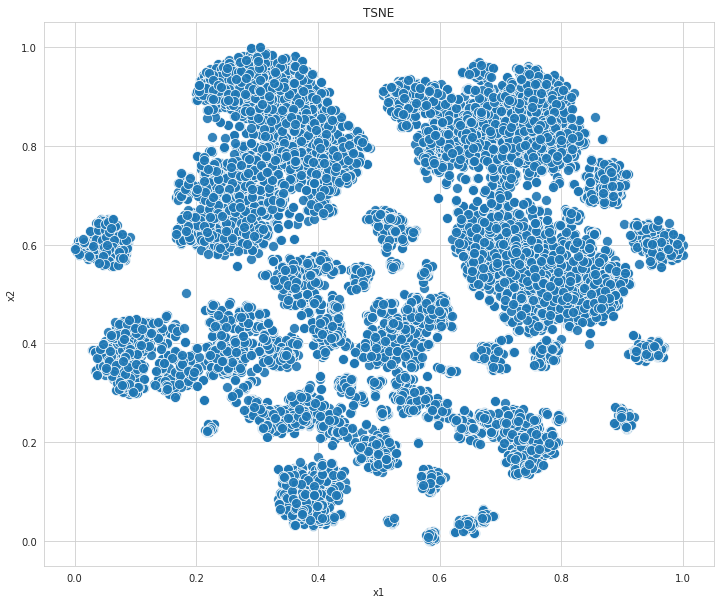
\includegraphics{/media/mmozolewski/m.mozolewski@gma/Documents/Doktorat/Parisa/xai-survey/article/example1-clustering-products-fashion-tex/output_57_1}
    \caption{}
    \label{fig:}
\end{figure}
\begin{figure}
    \centering
    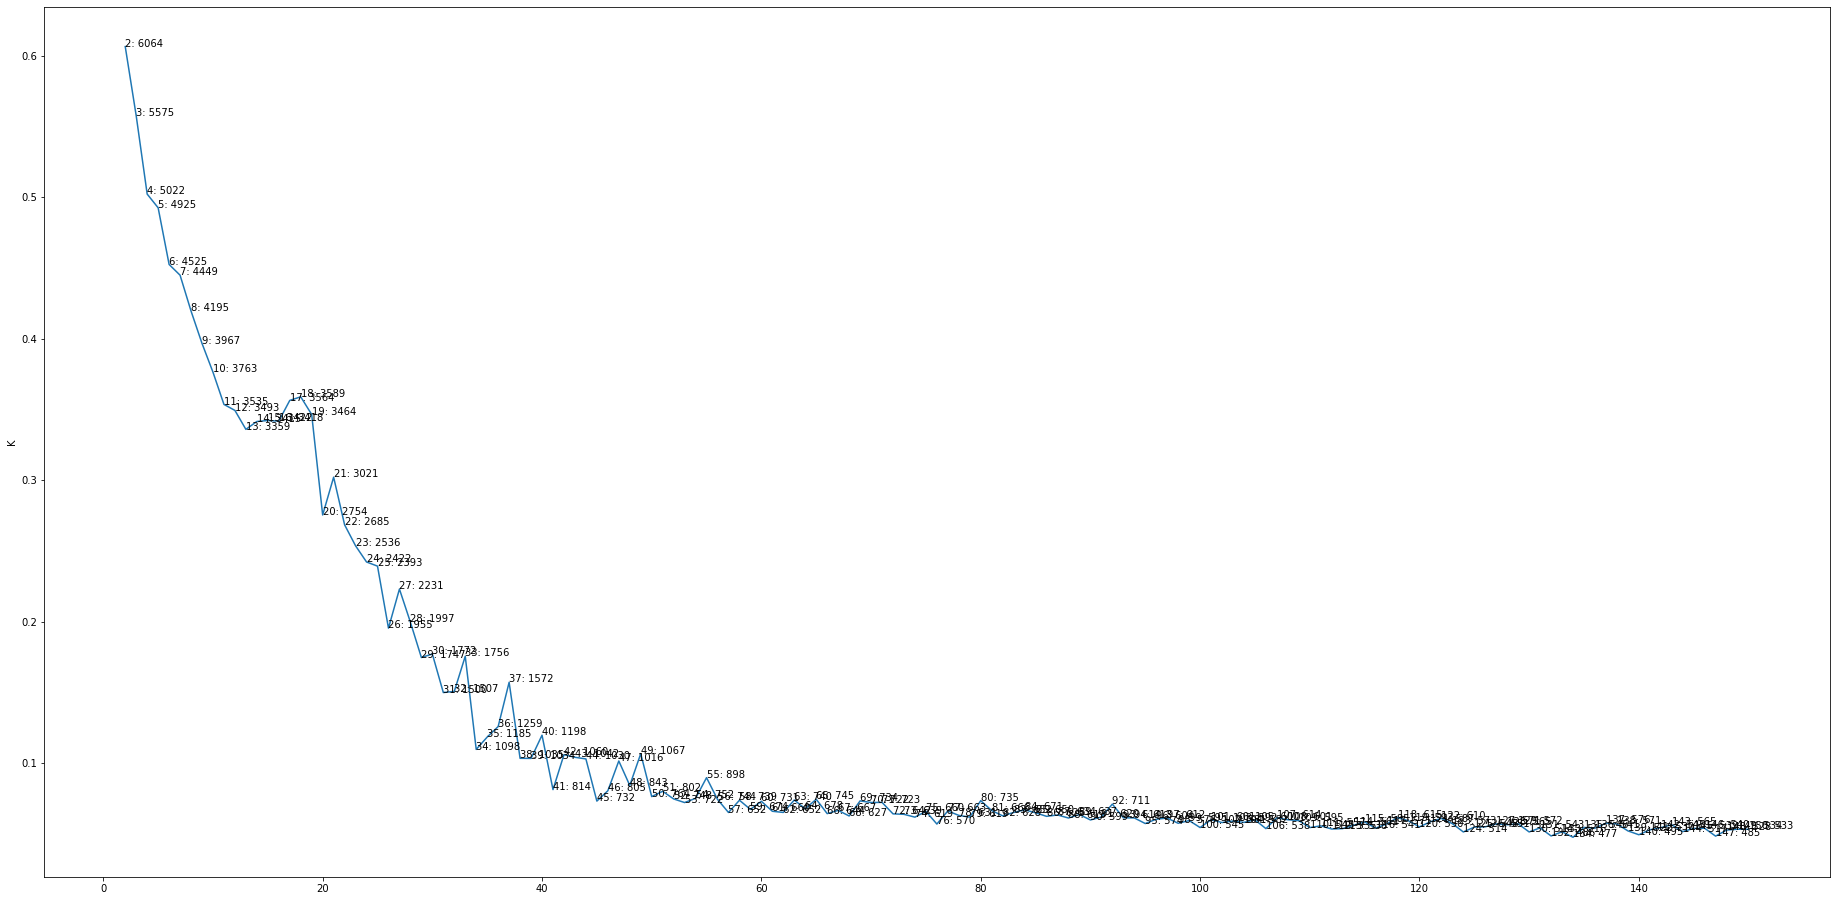
\includegraphics{/media/mmozolewski/m.mozolewski@gma/Documents/Doktorat/Parisa/xai-survey/article/example1-clustering-products-fashion-tex/output_58_0}
    \caption{}
    \label{fig:}
\end{figure}

Textual data was processed as follows:


\section{Summary}
SEO
visual modality
- hierarchical clustering
- Latent Dirichlet Allocation
%:)

\begin{acknowledgments}
  Thanks to the developers of ACM consolidated LaTeX styles
  \url{https://github.com/borisveytsman/acmart} and to the developers
  of Elsevier updated \LaTeX{} templates
  \url{https://www.ctan.org/tex-archive/macros/latex/contrib/els-cas-templates}.  
\end{acknowledgments}

%%
%% Define the bibliography file to be used
\bibliography{sample-ceur}





\end{document}

%%
%% End of file
